\begin{frame}[fragile]
	\frametitle{Algorithm}
	\framesubtitle{Pseudocode}
	\begin{center}
		\begin{algorithmic}
			\STATE $updateAccelerations()$
			\FOR {$counter = 0 \to iterations$}
			    \STATE $updatePositions()$
			    \STATE $updateAccelerations()$
			    \STATE $updateVelocities()$
			\ENDFOR
		\end{algorithmic}
	\end{center}
\end{frame}

\frame
{
    \frametitle{Algorithm}
    \framesubtitle{Development phases}
    \begin{itemize}
        \item Serial implementation.
        \item Profiling.
        \item Alternative implementations.
        \item Comparison.
    \end{itemize}
}


\begin{frame}[fragile]
    \frametitle{Algorithm}
    \framesubtitle{Profiling}
     \begin{itemize}
         \item Using \texttt{gprof}.
     \end{itemize}
     \begin{table}[h!t]
        \centering
        \scriptsize
        \begin{tabular}{|c|c|c|c|c|}
           \hline
           {\bf \% Time } & {\bf self seconds} & {\bf calls} & {\bf total ms/call} & {\bf name} \\\hline
             99.74   &  51.20   &  1002   &  51.10  & updateAccelerations() \\\hline
              0.08   &   0.04   &  1001   &   0.04  & updateVelocities()\\\hline
              0.02   &   0.01   &  1001   &   0.01  & updatePositions()\\\hline
              0.00   &   0.00   &     1   &   0.00  & checkAndInit(int, char const**)\\\hline
        \end{tabular}
        \caption{Serial implementation, using 1024 bodies}
     \end{table}
\end{frame}

\frame
{
    \frametitle{Algorithm}
    \framesubtitle{Alternative implementations - OpenMP}
    \begin{columns}
        \begin{column}{0.5\textwidth}
            \blue{Pros}
            \begin{itemize}
                \item Data decomposition automatically.
                \item A couple of extra code-lines.
                \item Allows fine and coarse grained algorithms.
            \end{itemize}
        \end{column}
        \begin{column}{0.5\textwidth}
            \red{Cons}
            \begin{itemize}
                \item Missing error handling.
                \item Invisible synchronization.
                \item Lack of thread-processor mapping.
            \end{itemize}
        \end{column}
    \end{columns}
}

\frame
{
    \frametitle{Algorithm}
    \framesubtitle{Alternative implementations - POSIX threads}
    \begin{columns}
        \begin{column}{0.5\textwidth}
            \blue{Pros}
            \begin{itemize}
                \item Synchronization handling.
                \item Build your own mechanism.
            \end{itemize}
        \end{column}
        \begin{column}{0.5\textwidth}
            \red{Cons}
            \begin{itemize}
                \item Needs parallel programming knowledge.
                \item Critical code intervention.
            \end{itemize}
        \end{column}
    \end{columns}
}
\frame
{
    \frametitle{Algorithm}
    \framesubtitle{Alternative implementations - CUDA}
    \begin{columns}
        \begin{column}{0.5\textwidth}
            \blue{Pros}
            \begin{itemize}
                \item Dedicated device.
                \item Fast shared memory access.
                \item High number of cores.
            \end{itemize} 
        \end{column}
        \begin{column}{0.5\textwidth}
            \red{Cons}
            \begin{itemize}
                \item Needs specialized architecture knowledge.
                \item New programming structure.
                \item Price/Benefit.
            \end{itemize}
        \end{column}
    \end{columns}
}

\frame
{
    \frametitle{Algorithm}
    \framesubtitle{Architecture}
    \begin{figure}
        \centering
        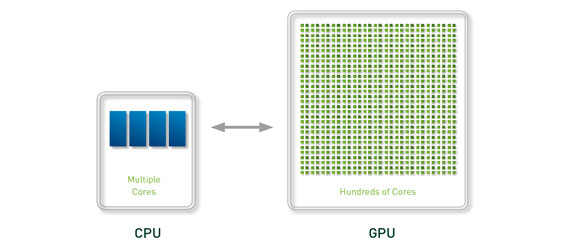
\includegraphics[width=0.7\textwidth]{img/architecture}
        \caption{CPU and GPU architecture}
    \end{figure}
}
